%% LyX 2.4.2.1 created this file.  For more info, see https://www.lyx.org/.
%% Do not edit unless you really know what you are doing.
\documentclass[12pt]{article}
\PassOptionsToPackage{natbib=true}{biblatex}
\usepackage[T1]{fontenc}
\usepackage[utf8]{inputenc}
\usepackage{verbatim}
\usepackage{amsmath}
\usepackage{graphicx}
\usepackage{geometry}
\geometry{verbose,tmargin=3cm,bmargin=2cm,lmargin=1.5cm,rmargin=1.5cm}

\makeatletter

%%%%%%%%%%%%%%%%%%%%%%%%%%%%%% LyX specific LaTeX commands.
%% Because html converters don't know tabularnewline
\providecommand{\tabularnewline}{\\}

\@ifundefined{date}{}{\date{}}
\makeatother

\usepackage[english]{babel}
\usepackage[style=authoryear,uniquename=false,uniquelist=false]{biblatex}
\addbibresource{minibib.bib}
\begin{document}
\title{Example for R package \texttt{lyxport}}
\author{Mark Bravington, November 2024}

\maketitle
This document tests the abilities of \texttt{lyxport} to handle cross-referencing
and numbering and citations and appendices and so on. You can try
exporting it from LyX to MSWord, both with LyX's built-in converter,
and with \texttt{lyxport}. The document evolved from my original tests
and notes, and so the contents might seem a bit odd... but this is
all about style, not content!

\section{Biblio info: housekeeping}

Somewhere in this file, there needs to be information on how to format
the bibliography, ie what CSL style file to use. Like this:

%% CSL ./journal-of-applied-genetics.csl
%% NB this is a "local" copy just for demo; better to install globally

Because it's a local bibliography (just a file in the same folder
as this one--- note the ``./'') I also need to make sure it gets
passed on during the export process, like this: (Look at ``lyxport-docu''.)

\begin{comment}
\verbatiminput{journal-of-applied-genetics.csl}
\end{comment}

If the CSL was installed ``globally'' (see ``lyxport-docu''...)
I wouldn't need that.

If you export this file to PDF (or just do Document->View) you won't
see the ERT or the verbatim-include. In fact the same goes for exporting
to MSWord, but they have to be in the LyX source for export-to-MSWord
to work properly.

\section{A bit of maths and so on}

Matrices/arrays, nested, and w/wout delimiters (which lead to different
Latex structures):

\begin{gather}
\left(\begin{array}{c}
\begin{array}{cc}
a & b\\
c & d
\end{array}\\
y\\
\pi
\end{array}\right)=0\label{eq:lab1}\\
\alpha+\beta\nonumber 
\end{gather}

What about an xrefed list?
\begin{enumerate}
\item \emph{I} am first\label{enu:I-am-first}
\begin{enumerate}
\item \emph{and} I have a sub-item\label{enu:sub1}
\end{enumerate}
\item But, dear item \ref{enu:I-am-first}, \emph{I} have the last word\label{enu:But-I-have}!
\item No you don't, item~\ref{enu:But-I-have}... I have been subcontracted
by sub-item \ref{enu:sub1}:)
\end{enumerate}
Here's a bona fide equation (which doesn't translate properly to ODT,
but is OK in MSWord):

\begin{equation}
\log f\left(Y,\beta|X;\lambda,\theta\right)=\log f\left(Y|X\beta;\theta\right)+\frac{1}{2}\log\|\lambda S\|_{+}-\frac{1}{2}\lambda\beta^{\top}S\beta\label{eq:beetle}
\end{equation}

Just to say again: the Bayesian framework leads to this log-probability
(up to an additive constant):
\begin{gather}
\log f\left(Y,\beta|X;\lambda,\theta\right)=\log f\left(Y|X\beta;\theta\right)+\frac{1}{2}\log\|\lambda S\|_{+}-\frac{1}{2}\lambda\beta^{\top}S\beta\label{eq:smoo-jt-lglk}
\end{gather}
where $\|\lambda S\|_{+}$ is a Thing. Let's reference the equation:
(\ref{eq:smoo-jt-lglk})! Or its predecessor, eqn (\ref{eq:beetle}).
(Or both of them: eqns (\ref{eq:beetle}) and (\ref{eq:smoo-jt-lglk})).

Lots of things didn't work for equation-labelling, such as tag-star
alignment.

This version is LyX's \textquotedbl Displayed equation\textquotedbl ,
which is only useful for a single line IMO. It maps to \textquotedbl\textbackslash equation\textquotedbl{}
if numbered/labeled, or \textquotedbl\textbackslash equation{*}\textquotedbl{}
if neither.

\[
a+b
\]

With a number 

\begin{equation}
x+y
\end{equation}

Just testing a fwd xref here, to section~\ref{sec:Stars}...

\section{Sections}\label{sec:tags}

The quick brown fox jumped over the lazy dog. Here is a tabular version,
Table~\ref{tab:Animals}; remember that you gotta \emph{refer} to
a table (ie xref it) somewhere, otherwise numbering won't work right.

\begin{table}[h]
\caption{Animals}\label{tab:Animals}

\begin{tabular}{|c|c|c|}
\hline 
Animal\textbackslash attribute & Colour & Velocity\tabularnewline
\hline 
\hline 
Fox & Brown & Fast\tabularnewline
\hline 
Dog & ? & Slow\tabularnewline
\hline 
\end{tabular}
\end{table}


\subsection{testy subsec}\label{subsec:testy-subsec}

Now is the time for all good men to come to the aid of the party.

\section{Stars}\label{sec:Stars}

Cross ref to sections~\ref{sec:tags} and \ref{subsec:testy-subsec}.
Now checking starred and unstarred gathers. Unlabeled first:
\begin{gather*}
\sin\pi\\
0+0
\end{gather*}

now labeled:
\begin{gather}
\cos\phi\label{eq:cosphi}\\
xxx\nonumber \\
1+1\nonumber 
\end{gather}

And to see whether we can get all-nonumber:
\begin{gather*}
\text{line 1}\\
\text{line 2}
\end{gather*}

and to see if the numbers are working alright, a simple one:

\begin{gather}
e^{i\pi}=-1\label{eq:euler}
\end{gather}

And let's get jiggy with a figgy, Figure~\ref{fig:oobl-goobl} in
fact:

\begin{figure}[h]
\caption{oobl goobl}\label{fig:oobl-goobl}

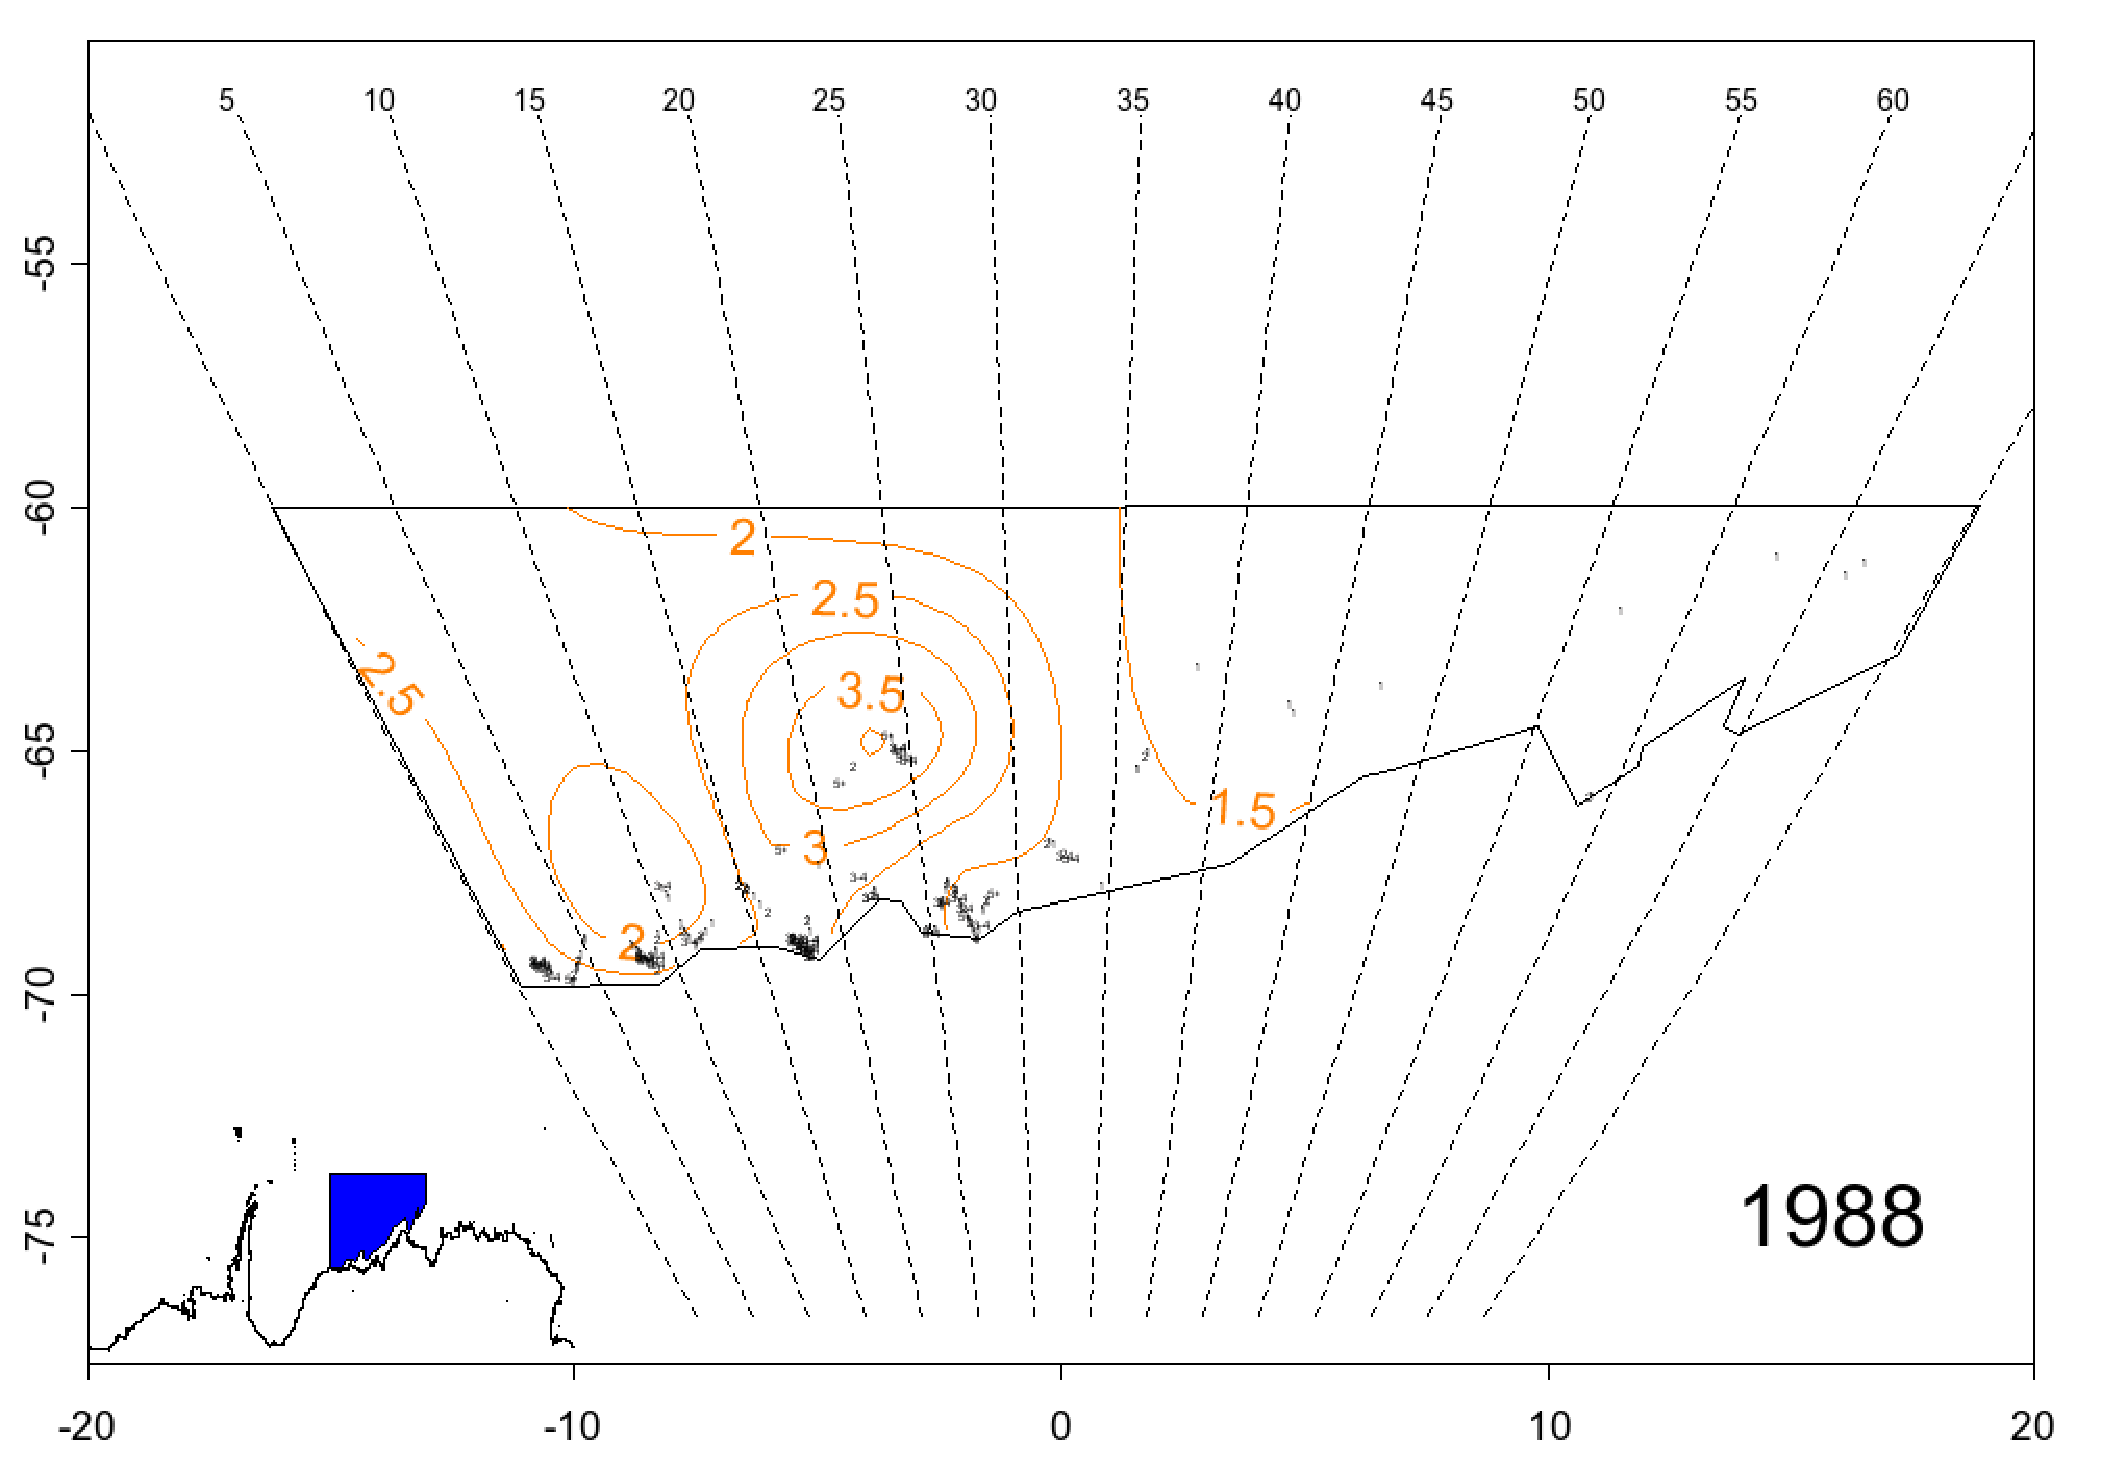
\includegraphics[scale=0.2]{nice-gs-Rplot009}
\end{figure}


\section{Citations}

Words and more via \citet{AAAtest} using citet or \citet{AAAtest,BBBtest}. 

Or we can drop all parens and commas, with citealt: eg \citealt{AAAtest,DDDtest,CCCtest,BBBtest}
or \citealt{AAAtest}. Note that I have suppressed citation silliness
in PDF with Biblatex options \texttt{uniquename=false} and \texttt{uniquelist=false}.
For MSWord, the default behaviour of \texttt{lyxzip2word()} is to
do the same thing; see Lyxport's LyX help if you don't want that.

%% tidy_initials timid

We can also auto-put the whole thing directly into parens, via citep
\citep{AAAtest} or \citep{AAAtest,BBBtest}.

This is my favourite: citealp, with commas but without its own parentheses.
I have helpfully added braces for, errr, clarity: \{\citealp{AAAtest}\}
or \{\citealp{AAAtest,BBBtest,CCCtest}\}\printbibliography


\appendix

\section{I am the title of an Appendix!}

and \emph{I} am an equation within it, eqn (\ref{eq:not3}) to be
precise:

\begin{gather}
1+1\neq3\label{eq:not3}
\end{gather}

BTW here's a ref to the same eqn with built-in parens: eqn~(\ref{eq:not3}).
What about sections within an appendix?

\subsection{Here's one!}

There's not much to me, though. Just Table~\ref{tab:apxtab}, to
check tab numbering in Apxes:

\begin{table}[h]
\caption{What is my name?}\label{tab:apxtab}

\begin{tabular}{|c|c|}
\hline 
black & white\tabularnewline
\hline 
\end{tabular}
\end{table}


\section{Things that don't work right}

This section is \emph{hugely }incomplete!

Cases: see eqn~\ref{eq:precase}, with a superfluous right-paren
(in MSWord at least).
\begin{gather}
\sin\pi=0\label{eq:precase}\\
\begin{cases}
x>0 & \alpha\\
x<0 & \beta
\end{cases}\nonumber 
\end{gather}

\end{document}
